\documentclass{simple}

\usepackage{subcaption}

\title[Despre congurență]{Despre congruență}
\institute{InfoEducație 2019, Gălăciuc, Vrancea}
\author[Răzvan Deaconescu]{Răzvan Deaconescu \\
razvan.deaconescu@cs.pub.ro}
\date{3 august 2019}

\begin{document}

\frame{\titlepage}

\begin{frame}{Exercițiu}
  \centering
  \pause
  \Large{3 cuvinte care te definesc} \\
  \pause
  \vspace{1cm}
  \Large{curator, energizer, builder}
\end{frame}

\begin{frame}{Traian Băsescu}
  \begin{itemize}
    \pause
    \item dezbatere cu Mircea Geoană și Dumitru (Mitică) Dragomir (2004, primărie București)
    \pause
    \item ,,Mă, Mitică, \ldots''
  \end{itemize}
\end{frame}

\begin{frame}{Ce înseamnă că ești congruent?}
  \centering
  \Large
  \pause
  te comporți, afișezi așa ,,cum ești tu''\\
  \pause
  te simți bine în propria-ți piele\\
  \pause
  ce afișezi este compatibil cu felul în care ești\\
  \pause
  congruența îți spune ce lucruri să \textbf{NU} faci\\
  \pause
  compensată de bun simț și disciplină
\end{frame}

\begin{frame}{Congruență, fii tu însuți, onestitate}
  \centering
  \pause
  mai mult decât un singur \textbf{sine}; suntem maleabili, avem nuanțe \\
  \pause
  amibă: un nucleu (miez, \textit{core}) și pseudopode, aspecte ale personalității \\
  \pause
  ,,Onestitatea este bună pentru conștiință dar rea pentru carieră.'' \\
  \pause
  onestitatea = afișezi tot \\
  \pause
  congruența = afișezi compatibil cu tine, cu miezul tău
\end{frame}

\begin{frame}[fragile]{Lucifer}
  \begin{figure}
    \centering
    
\includegraphics[width=0.55\linewidth]{img/lucifer-wings}
  \end{figure}
  \begin{figure}
    \centering
    
\includegraphics[width=0.55\linewidth]{img/lucifer-devil-form}
  \end{figure}
\end{frame}

\begin{frame}{Congruență: Teoria psihologică}
  \begin{itemize}
    \pause
    \item Carl Rogers
    \pause
    \item \url{https://www.simplypsychology.org/carl-rogers.html}
    \pause
    \item \textit{Carl Rogers (1959) believed that humans have one basic motive, that is the tendency to self-actualize - i.e., to fulfill one's potential and achieve the highest level of ``human-beingness'' we can.}
    \pause
    \item \textit{that for a person to ``grow'', they need an environment that provides them with genuineness (openness and self-disclosure), acceptance (being seen with unconditional positive regard), and empathy (being listened to and understood).}
    \pause
    \item \textit{This means that self-actualization occurs when a person's ``ideal self'' (i.e., who they would like to be) is congruent with their actual behavior (self-image).}
  \end{itemize}
\end{frame}

\begin{frame}{Congruență: Teoria psihologică}
  \centering
  \pause
  \Large{I am vs I should be}
  \pause
  \begin{figure}
    \centering
    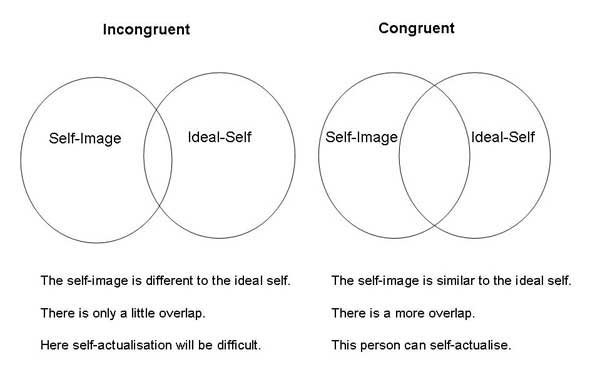
\includegraphics[width=0.8\textwidth]{img/congruence}\\
    \scriptsize{\url{https://www.simplypsychology.org/carl-rogers.html}}
  \end{figure}
\end{frame}

\begin{frame}{De ce e bine să fii congruent?}
  \begin{itemize}
    \pause
    \item autenticitate, naturalețe, comportament ingenuu
    \pause
    \item \textit{feel good in your own skin}
    \pause
    \item îi relaxează pe ceilalți, ajungi mai ușor la ei, ești credibil
    \pause
    \item ethos / pathos / logos; ethos: credibilitate
    \pause
    \item încredere de sine (\textit{confidence})
    \pause
    \item evoluție, creștere, \textit{self-actualization}
  \end{itemize}
\end{frame}

\begin{frame}{Self-actualization}
  \begin{figure}
    \centering
    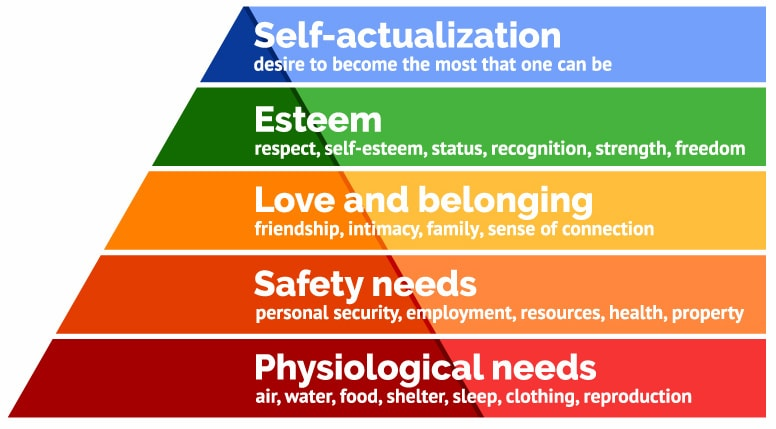
\includegraphics[width=0.8\textwidth]{img/maslow-hierarchy-of-needs}\\
    \scriptsize{\url{https://www.simplypsychology.org/maslow.html}}
  \end{figure}
\end{frame}

\begin{frame}{Ce cauzează incongruență?}
  \begin{itemize}
    \pause
    \item vrei să dai bine
    \pause
    \item vrei prea mult prea repede
    \pause
    \item presiune socială: ,,trebuie să faci așa, trebuie să fii ca ceilalți''
    \pause
    \item anti-presiune socială: ,,fac pe dos, sunt unic, diferit''
    \pause
    \item teama de a fi judecat, ostracizat
    \pause
    \item nu te cunoști, nu știi unde vrei să ajungi
    \pause
    \item superficialitate, accent pe aspecte materiale, fizice, concrete
    \pause
    \item lipsă de timp
  \end{itemize}
\end{frame}

\begin{frame}{Nuanțe}
  \begin{itemize}
    \pause
    \item cineva nu este complet X sau complet Y, există nuanțe
    \item nu avem alb negru, 0-1; avem 0-10, avem grade
    \item cineva este acum gradul 5 de X, în altă situație este 4 de X
    \pause
    \item suntem maleabili
    \item suntem dinamici, evoluăm; ne propunem să ajungem undeva
  \end{itemize}
\end{frame}

\begin{frame}{Cum ajungi congruent?}
  \begin{itemize}
    \pause
    \item \textit{listen to your gut}
    \pause
    \item \textit{know yourself}
    \pause
    \item nu-ți fie teamă de părerea altora
    \pause
    \item ai răbdare
    \pause
    \item acceptă imperfecțiunile
    \pause
    \item \textit{maximize strengths, minimize weaknesses}
  \end{itemize}
\end{frame}

\begin{frame}{Pași concreți}
  \begin{itemize}
    \pause
    \item solitudine, meditație, \textit{daydreaming}
    \pause
    \item discuții pe subiecte contondente: sex, căsătorie, religie, politică, educație, sărăcie, pedeapsa cu moartea, climă, minorități, legalizare droguri, prostituție
    \pause
    \item aveți opinii, exprimați opinii
    \pause
    \item relații intime
    \pause
    \item țineți prezentări, prelegeri, tutoriale, cursuri
    \pause
    \item obțineți feedback (anonim și autentic)
    \pause
    \item vorbiți pe șleau, chiar dur; îi va relaxa pe alții să vorbească pe șleau și dur
    \pause
    \item caută mentori
    \pause
    \item fii mentor
  \end{itemize}
\end{frame}

\begin{frame}{Unde să găsești onestitate?}
3 types of people who are honest:\\
1. Children\\
2. Drunks\\
3. Anons\\
  \hfill{\textit{Black Label Logic (Twitter)}}
\end{frame}

\begin{frame}{În loc de final}
  \centering
  \pause
  \Large{Exercițiu: 3 cuvinte care te definesc} \\
  \pause
  \Large{Nu e ușor.} \\
  \pause
  \Large{Congruența nu înseamnă imagine statică. Evoluezi, te schimbi, te auto-actualizezi.}
\end{frame}

\begin{frame}{Resurse și recomandări}
  \begin{itemize}
    \item slide-urile prezentării: \url{https://www.slideshare.net/razvandeaconescu/}
    \item \url{https://www.simplypsychology.org/carl-rogers.html}
    \item \url{https://quillette.com}
    \item Intellectual Dark Web
    \item Bill George: Authentic Leadership
    \item Bill George: True North
  \end{itemize}
\end{frame}

\end{document}
